\documentclass[12pt]{article}
%Librerías
\usepackage[utf8]{inputenc}
\usepackage[spanish,mexico]{babel}
% Comando para obtener el nombre del mes actual en español
\newcommand{\monthname}{%
  \ifcase\month\or enero\or febrero\or marzo\or abril\or mayo\or junio\or julio\or agosto\or septiembre\or octubre\or noviembre\or diciembre\fi}

\usepackage[scaled]{helvet} % Carga la fuente similar a Arial
\usepackage[T1]{fontenc}
\usepackage{lmodern} 
\usepackage{anyfontsize}
\usepackage{float}
\usepackage{pdflscape}
\usepackage[
    a4paper,
    left=2.5cm,
    right=2.5cm,
    top=2.5cm,
    bottom=2.5cm
]{geometry}

% --- Gráficos y Colores ---
\usepackage[table,xcdraw]{xcolor} % Carga xcolor una sola vez
\usepackage{graphicx}
\usepackage{tikz}
\usetikzlibrary{calc,arrows}
\usepackage{float}
\usepackage{caption}

% --- Tablas y Organización ---
\usepackage{booktabs}
\usepackage{array}
\usepackage{longtable}
\usepackage{multicol}

\usepackage{fancyhdr}
\pagestyle{fancy}
\fancyhf{} % Limpia cualquier encabezado/pie predeterminado
\renewcommand{\headrulewidth}{0pt} % Elimina la línea negra por defecto de LaTeX

% --- Configuración de Líneas Flotantes ---
\usepackage{fancyhdr}
\pagestyle{fancy}
\fancyhf{} 
\renewcommand{\headrulewidth}{0pt}


\usepackage{titlesec}

% --- Configuración de Secciones (Todas a 12pt) ---

% Nivel 1: SECCIÓN (12pt, Negrita)
\titleformat{\section}
  {\normalfont\fontsize{12}{14}\bfseries}
  {\thesection.}
  {1em}
  {}

% Nivel 2: SUBSECCIÓN (12pt, Negrita)
\titleformat{\subsection}
  {\normalfont\fontsize{12}{14}\bfseries}
  {\thesubsection.}
  {1em}
  {}

% Nivel 3: SUBSUBSECCIÓN (12pt, Negrita y quizás Itálica para diferenciar)
\titleformat{\subsubsection}
  {\normalfont\fontsize{12}{14}\bfseries\itshape}
  {\thesubsubsection.}
  {1em}
  {}

\usepackage{tocloft}

% Configura el título del índice "Índice" o "Tabla de Contenidos" a 12pt y Negrita
\renewcommand{\cfttoctitlefont}{\normalfont\fontsize{12}{14}\bfseries}

% Configura las Secciones en el índice (Nivel 1)
\renewcommand{\cftsecfont}{\normalfont\fontsize{12}{14}\selectfont}     % Texto
\renewcommand{\cftsecpagefont}{\normalfont\fontsize{12}{14}\selectfont} % Número de página

% Configura las Subsecciones en el índice (Nivel 2)
\renewcommand{\cftsubsecfont}{\normalfont\fontsize{12}{14}\selectfont}
\renewcommand{\cftsubsecpagefont}{\normalfont\fontsize{12}{14}\selectfont}

% Configura las Sub-subsecciones en el índice (Nivel 3)
\renewcommand{\cftsubsubsecfont}{\normalfont\fontsize{12}{14}\selectfont}
\renewcommand{\cftsubsubsecpagefont}{\normalfont\fontsize{12}{14}\selectfont}

% Opcional: Si quieres puntos suspensivos en las secciones (LaTeX por defecto no los pone en nivel 1)
\renewcommand{\cftsecdotsep}{\cftdotsep}

% --- Configuración para Lista de Figuras ---
\renewcommand{\cftloftitlefont}{\normalfont\fontsize{12}{14}\bfseries} % Título "Índice de Figuras"
\renewcommand{\cftfigfont}{\normalfont\fontsize{12}{14}\selectfont}     % Texto de la figura
\renewcommand{\cftfigpagefont}{\normalfont\fontsize{12}{14}\selectfont} % Número de página

% --- Configuración para Lista de Tablas ---
\renewcommand{\cftlottitlefont}{\normalfont\fontsize{12}{14}\bfseries} % Título "Índice de Tablas"
\renewcommand{\cfttabfont}{\normalfont\fontsize{12}{14}\selectfont}     % Texto de la tabla
\renewcommand{\cfttabpagefont}{\normalfont\fontsize{12}{14}\selectfont} % Número de página

\usepackage{caption}

% Configuración Global APA 7 (Títulos arriba para todo)
\captionsetup{
    position=above,       % Fuerza el título arriba
    labelfont=bf,         % "Figura 1" o "Tabla 1" en Negrita
    textfont=it,          % El texto descriptivo en Cursiva
    labelsep=newline,     % Salto de línea entre "Figura 1" y el título (Estilo APA 7)
    justification=justified,
    singlelinecheck=false, % Alineación a la izquierda
    skip=10pt             % Espacio entre el título y la imagen/tabla
}

\usepackage{setspace}

% Aplicar interlineado 1.5 a todo el documento
\onehalfspacing

% --- Texto de relleno y Enlaces ---
\usepackage{lipsum} 

% --- Bibliografía (APA 7 Estándar) ---
\usepackage{csquotes}
\usepackage[style=apa, backend=biber]{biblatex}
\addbibresource{references.bib}

% --- Configuración de Enlaces ---
\usepackage{hyperref}
\hypersetup{
    colorlinks=true,
    linkcolor=black,
    citecolor=blue,
    urlcolor=blue
}

% --- PARCHE FINAL SIN ERRORES (Todo azul, con espacio y fecha visible) ---
\DeclareFieldFormat{citehyperref}{\bibhyperref{\textcolor{blue}{#1}}}

% 1. Formato para los Nombres
\DeclareNameFormat{labelname:hyperref}{%
  \bibhyperref{\textcolor{blue}{%
    \ifcase\value{uniquename}%
      \usebibmacro{name:family}{\namepartfamily}{\namepartgiven}{\namepartprefix}{\namepartsuffix}%
    \or
      \usebibmacro{name:given-family}{\namepartfamily}{\namepartgiveni}{\namepartprefix}{\namepartsuffix}%
    \or
      \usebibmacro{name:given-family}{\namepartfamily}{\namepartgiven}{\namepartprefix}{\namepartsuffix}%
    \fi}}%
  \usebibmacro{name:andothers}}

% 2. Redefinición de los comandos de cita
\makeatletter

% Fix para \parencite: (Autor, Año)
\DeclareCiteCommand{\parencite}[\mkbibparens]
  {\usebibmacro{prenote}}
  {\printtext[citehyperref]{%
     \printnames{labelname}%
     \setunit{\printdelim{nameyeardelim}}%
     \printlabeldateextra}} % <--- Comando estándar para el año en APA
  {\multicitedelim}
  {\usebibmacro{postnote}}

% Fix para \textcite: Autor (Año)
\DeclareCiteCommand{\textcite}
  {\boolfalse{cbx:parens}}
  {\printtext[citehyperref]{\printnames{labelname}}%
   \setunit{\addspace}% <--- Espacio corregido
   \printtext[citehyperref]{%
     \ifnumequal{\value{citecount}}{1}{\bibopenparen}{}%
     \printlabeldateextra}} % <--- Comando estándar para el año en APA
  {\ifbool{cbx:parens}{\bibcloseparen\global\boolfalse{cbx:parens}}{}\multicitedelim}
  {\ifnumequal{\value{citecount}}{\value{citetotal}}{\bibcloseparen}{}\usebibmacro{postnote}}

\makeatother

% --- CONFIGURACIÓN PARA URLs DENTRO DE MÁRGENES ---
\usepackage{url}

% 1. Permitir que las URLs se rompan en números y caracteres especiales
\expandafter\def\expandafter\UrlBreaks\expandafter{\UrlBreaks%  
  \do\/\do\-\do\.\do\0\do\1\do\2\do\3\do\4\do\5\do\6\do\7\do\8\do\9\do\a\do\b\do\c\do\d\do\e\do\f\do\g\do\h\do\i\do\j\do\k\do\l\do\m\do\n\do\o\do\p\do\q\do\r\do\s\do\t\do\u\do\v\do\w\do\x\do\y\do\z\do\A\do\B\do\C\do\D\do\E\do\F\do\G\do\H\do\I\do\J\do\K\do\L\do\M\do\N\do\O\do\P\do\Q\do\R\do\S\do\T\do\U\do\V\do\W\do\X\do\Y\do\Z}

% 2. Forzar que las URLs usen la misma fuente que el documento (opcional pero recomendado)
\urlstyle{same}

    
\begin{document}

%%%%%%%%%%%%%%%%%%%%%%%%%%%
%%%%%%%%%%%%%%%%%%%%%%%%%%%
%%%%%%%%%%%%%%%%%%%%%%%%%%%

% --- INICIO DE CARÁTULA ---

%%%%%%%%%%%%%%%%%%%%%%%%%%%
%%%%%%%%%%%%%%%%%%%%%%%%%%%
%%%%%%%%%%%%%%%%%%%%%%%%%%%
\begin{titlepage}
    \sffamily % A partir de aquí, todo el texto será "Arial" (Helvetica)
\thispagestyle{empty} 

% DIBUJO DE LAS LÍNEAS (Solo para esta página)
    \begin{tikzpicture}[remember picture, overlay]
        % Línea superior a 1cm de los bordes
        \draw[thick, lightgray] 
            ([xshift=1cm, yshift=-1cm]current page.north west) -- 
            ([xshift=-1cm, yshift=-1cm]current page.north east);

        % Línea inferior a 1cm de los bordes
        \draw[thick, lightgray] 
            ([xshift=1cm, yshift=1cm]current page.south west) -- 
            ([xshift=-1cm, yshift=1cm]current page.south east);
    \end{tikzpicture}

\begin{center}
%    \vspace{1.0 cm}
        \scalebox{2.5}{ 
                \begin{minipage}{0.2\textwidth} 
                    \centering
                
\includegraphics[width=\textwidth]{images/Logo_UPS.png}
                \end{minipage}
            %}
        }

    \vspace{1.1cm}
        {\fontsize{22}{28}\selectfont \textbf{Universidad Politécnica Salesiana}} \\[0.3cm]
        {\fontsize{18}{22}\selectfont Sede Guayaquil}  

    \vspace{1.5cm}
    {\fontsize{14}{16}\selectfont {CARRERA: COMPUTACIÓN}} \\
    \vspace{1.8cm}
    {\fontsize{14}{16}\selectfont \textbf{ANTEPROYECTO}} \\
    \vspace{0.2cm}
    {\fontsize{12}{14}\selectfont {Previo a la obtención del título de Ingeniero en Ciencias de la Computación}} \\

    \vspace{2.1cm}
    {\fontsize{12}{14}\selectfont {TITULO}} \\
    \vspace{0.2cm}
    {\fontsize{12}{14}\selectfont {``Título con mayúsculas y minúsculas al menos 15 a 17 palabras y sin punto final''}} \\

    \vspace{1.9cm}
    {\fontsize{12}{14}\selectfont {AUTOR(ES)}} \\

    \vspace{0.2cm}
    {\fontsize{12}{14}\selectfont {Apellido1 Apellido2 Nombre1 Nombre2\\Apellido1 Apellido2 Nombre1 Nombre2}} \\

    \vspace{1.9cm}
    {\fontsize{12}{14}\selectfont {TUTOR}} \\
    {\fontsize{12}{14}\selectfont {Llerena Izquierdo Joe}} \\

\end{center}
\vspace{1.5cm} % Espacio ajustable para empujar la fecha hacia abajo
\begin{center}
    {\fontsize{12}{14}\selectfont Guayaquil, \monthname\ del \the\year}
\end{center}

\vfill % Empuja el contenido hacia arriba
\end{titlepage}
%%%%%%%%%%%%%%%%%%%%%%%%%%%
%%%%%%%%%%%%%%%%%%%%%%%%%%%
%%%%%%%%%%%%%%%%%%%%%%%%%%%

% Índices

%%%%%%%%%%%%%%%%%%%%%%%%%%%
%%%%%%%%%%%%%%%%%%%%%%%%%%%
%%%%%%%%%%%%%%%%%%%%%%%%%%%

\begin{singlespace} % Inicia espacio sencillo para todos los índices

% Agrupamos los índices para quitarles la numeración a la fuerza
\addtocontents{toc}{\protect\thispagestyle{empty}} 
%\pagestyle{empty} 

\tableofcontents
\newpage

\addtocontents{lof}{\protect\thispagestyle{empty}}
\listoffigures
\newpage

\addtocontents{lot}{\protect\thispagestyle{empty}}
\listoftables
\end{singlespace} % Aquí termina el espacio sencillo
\newpage

\pagestyle{plain}
\setcounter{page}{1} % <--- 3. Fuerza a que esta página sea la número 1
\pagenumbering{arabic} % Asegura que use números 1, 2, 3...

%%%%%%%%%%%%%%%%%%%%%%%%%%%
%%%%%%%%%%%%%%%%%%%%%%%%%%%
%%%%%%%%%%%%%%%%%%%%%%%%%%%

% --- CONTENIDO ---

%%%%%%%%%%%%%%%%%%%%%%%%%%%
%%%%%%%%%%%%%%%%%%%%%%%%%%%
%%%%%%%%%%%%%%%%%%%%%%%%%%%

\section{Tema del Trabajo de Titulación  }
%begin{center}
\noindent Título con mayúsculas y minúsculas al menos 15 a 17 palabras sin punto final evite comas dos puntos acrónimos mezclar inglés 
%\end{center}

\section{Antecedentes}
{\color{magenta}En este apartado se especificará cómo nace la idea, pregunta de investigación o problema de investigación; si existen trabajos previos y cualquier otra información que permita conocer aspectos previos al trabajo propuesto.}

Para todo anteproyecto (proyecto técnico o un artículo científico), los Antecedentes (también llamados Estado del Arte o Trabajos Relacionados) representa la redacción a manera de relatos, objetivo y formal \parencite{puga2023mapeo,Melendrez-Caicedo2022}, de aquella trayectoria que ha tenido el tema de investigación escogido, citando otros textos y que evidencian la necesaria justificación de tu investigación. En el primer párrafo debes colocar el conteto general (macro) que define el área tecnológica o científica actual. Describe la importancia del problema que quieres resolver como lo indican \textcite{Llerena-Izquierdo_Ayala-Carabajo_2022,10389227}. En el primer párrafo debe presentarse un escrito que describa tres preguntas -de forma narrativa-: 1. ¿Quiénes padecen o el problema a abordar? 2. ¿Cuánto les cuesta? 3. ¿Qué pasa si no hacemos nada?, y luego continuar de lo general a lo específico de la importancia del tema así como la novedad. El tono debe ser objetivo y formal, el verbo a usar es en presente (ej. ``Actualmente, el aprendizaje automático optimiza...''). Y debes citar 1 o 2 referencias con DOI de fuentes relevantes (WoS o Scopus) globales o estadísticas recientes. Evita usar Google Académico \parencite{llerena2025guia}. 

En el segundo párrafo colocas aquellos trabajos relacionados (lo que ya existe científicamente) con tu tema de acuerdo a los constructos (aquellas palabras clave que están en tu título). El contenido que vas a mencionar deben ser investigaciones similares a la tuya. No hagas una lista; agrupa autores que usen técnicas parecidas. El tono de tu texto debe ser analítico. El verbo a usar es en pasado (ej. ``López et al. (2023) implementaron un algoritmo...''). Aquí se usan muchas citas de forma obligatoria. Es el corazón de las citas. No hagas una lista de ``X dijo esto y Y dijo aquello''. Intenta compararlos. Por ejemplo,  ``Mientras que \textcite{Sanchez-Romero_Llerena-Izquierdo_2023} proponen un enfoque basado en la nube, \textcite{zambrano2024revision} sugiere que el procesamiento en el borde (edge computing) reduce la latencia en un 20\%.''.

En el tercer párrafo, se narra la brecha o vacío (lo que falta) del conocimiento. Es el párrafo más importante. Debes identificar qué no han hecho los autores anteriores o qué limitaciones tienen sus métodos. Es el párrafo más crítico. Debes explicar qué es lo que esos autores no resolvieron. El tono debe ser crítico pero respetuoso. Usa palabras claves como ``Sin embargo'', ``A pesar de estos avances'', ``No se ha evidenciado'', ``Existe una limitación en''. Al usar los verbos, estos deben estar en presente o presente perfecto (ej. ``Sin embargo, estas soluciones no consideran...'', ``Ha sido difícil lograr precisión en...'' o ``Sin embargo, los estudios previos no consideran las restricciones de infraestructura tecnológica en sectores rurales de la costa ecuatoriana...'') \parencite{molina2025gestion}. Aquí son pocas citas o ninguna (es tu análisis).

El cuarto párrafo debe enfocarse a tu propuesta (¿Qué hay de nuevo?), así en el contenido, respondes a la relevancia del tema escogido. Cómo tu proyecto técnico o artículo va a llenar ese vacío \parencite{Llerena-Izquierdo2025}. El tono debe ser propositivo y decidido.
Al usar los verbos estos deben estar en futuro (para Anteproyectos) o Presente (para Artículos finalizados). Ej: ``Este proyecto desarrollará un modelo que...'', ``Para resolver esta brecha, el presente proyecto técnico plantea una arquitectura que... [tu novedad]'' o ``Siguiendo la línea de investigación de \textcite{izquierdo2025hacia} sobre minería de datos, este proyecto propone aplicar dichas técnicas pero enfocadas específicamente en...''. 

Cada subsección debe definir el pasado y presente de dicho concepto que se identifca en la palabra clave del título \parencite{Puma-Rodriguez2025}. Las preguntas clave que debes responder en toda esta sección, permiten al revisor tener una idea, alcance y conocimiento para que apruebe tu tema, deben quedar claras, ¿Es relevante tema? Sí, porque afecta a X industria o sector.
¿Qué hay de nuevo? No estoy inventando la rueda, estoy mejorando el rodamiento (ej. mayor velocidad, menor consumo de memoria, mejor precisión en datasets locales de Ecuador) \parencite{10442311,10389227}.

Los elementos visuales y formato de las subsecciones, tienen importancia en los anteproyectos y el tamaña o extensión de este es de 5-10 páginas \parencite{10.1007/978-3-031-98890-5_3}. El flujo de párrafos es continuo, evite usar viñetas o numerales dentro las secciones o subsecciones, así como usar inteligencia artificial generativa para escribir tus propios análisis y pensamientos \parencite{Ayala-Carabajo2026,guerrero2025integracion}. En artículos de alto impacto se suelen dividir por temas o constructos identificados (la sección de antecedentes) y que corresponden aquellas palabras clave que se encuentran en el título (ej. 2.1 Procesamiento de Lenguaje Natural, 2.2 Algoritmos de Clasificación).
Para las figuras o tablas según el formato de la enntidad que lo solicita, sigue con una numeración continua en todo el documento, por ejemplo el formato APA 7 \parencite{JacomeMarmol2025,guerrero2025integracion}. Recuerda, una tabla es una tabla, no puedes hacer imagen a una tabla. La tablas, son altamente recomendadas debes crearlas aunque sean de otro lugar o no haya cómo editarlas (no copiarlas) debes crearla. Una tabla comparativa de trabajos previos siempre debes utilizar, (donde pongas en sus columnas: Autor o citar la referencia, Técnica, Ventaja, Limitación), es lo que más valoran los revisores \parencite{10.1007/978-3-031-70760-5_37}.

Las figuras solo ayudan a explicar la arquitectura de una solución existente que vas a mejorar \parencite{Lopez-Chila2025}. No uses figuras decorativas. La figura principal del proyecto o artículo científico debe ser aquella que muestre todo el proceso de desarrollo. Una figura vale más que 100 palabras.
Finalmente el uso de citas y verbos deben seguir un formato. Para citas, deben de ser de artículos científicos de los últimos 5 años (bases de datos como IEEE Xplore, ACM, Scopus). Cita trabajos que hayan realizado tus profesores de la carrera, así ayudas a la visualización de trabajos de la universidad. Evita blogs o Wikipedia. Finalmente, los verbos o el tono, siempre en tercera persona (ej. ``Se observó'', ``Se propone'') o, si el estilo lo permite, nosotros formal (``Proponemos''). Nunca digas ``Yo creo'' o ``Yo hice''.

\section{Justificación}
{\color{magenta}Explica de forma breve y concisa la problemática profesional que se aborda y destaca el objetivo de investigación del mismo.}
La Justificación es, posiblemente, la sección más importante para ``vender'' tu proyecto al comité. Mientras que los antecedentes dicen qué han hecho otros, la justificación explica por qué es imprescindible que tú hagas este trabajo ahora.
Debes demostrar la conveniencia y los beneficios del proyecto. Debes convencer al lector de que existe un problema real (que has encontrado en la literatura) y que tu solución es viable, necesaria y aporta valor (técnico, social o institucional). Esta sección debe ser de tres a cuatro párrafos.
En el primer párrafo va la justificación técnica (el ``Cómo''), explica por qué la tecnología o metodología que elegiste es la correcta.
Ejemplo: ``Desde una perspectiva técnica, el uso de [Aprendizaje Profundo/Minería de Datos] permite procesar volúmenes de información que los métodos tradicionales no alcanzan...''.

El segindo párrafo, va la justificación social/institucional (el ``Quién''). ¿Quién se beneficia? (Estudiantes, la UPS, una empresa, el sector salud). Ejemplo: ``La implementación de esta plataforma beneficiará directamente a los estudiantes de la Facultad de Ingeniería, reduciendo el tiempo de...''.

El tercer párrafo, va la justificación teórica o de innovación (el ``Aporte''). ¿Qué conocimiento nuevo genera? ¿O qué problema específico resuelve que otros no hicieron?, ejemplo: ``Este proyecto aporta una nueva metodología de análisis que no ha sido explorada en el contexto local...''.

El cuarto párrafo, describes el impacto y factibilidad. Cierra diciendo que el proyecto es realizable (tienes los datos, el software y el apoyo). Un estudiante debe tener en mente estas cuatro preguntas. Si tu texto las responde, la justificación es sólida: ¿Para qué sirve? (Utilidad), ¿Por qué es importante? (Relevancia), ¿Qué problema real resuelve? (Resolución), ¿Es factible realizarlo? (Viabilidad).
La extensión del contenido va entre media página y una página completa. No debe ser tan larga como los antecedentes. El tono debe ser persuasivo pero objetivo. No uses opiniones personales (``Yo creo que es bueno''), usa hechos demostrables .
El uso de verbos deben denotar acción y beneficio:
Contribuir, optimizar, facilitar, fortalecer, reducir, proveer, sistematizar, innovar.

{\color{blue} La presente investigación se justifica por la necesidad crítica de fortalecer la seguridad en las arquitecturas modernas de comunicación de datos. A medida que las organizaciones adoptan GraphQL para optimizar la eficiencia en el intercambio de información, emergen vulnerabilidades específicas tales como la sobreexposición de datos y las consultas no controladas, las cuales representan un riesgo significativo para la integridad institucional.

Desde una perspectiva técnica, este proyecto es fundamental ya que propone la integración del modelo de Seguridad Zero Trust (Confianza Cero) en el desarrollo de APIs. La implementación de mecanismos de autenticación continua y control de acceso granular permitirá mitigar riesgos de accesos no autorizados e inyecciones de consultas, resolviendo las limitaciones de los enfoques de seguridad tradicionales que resultan insuficientes para sistemas distribuidos y microservicios.

En el ámbito práctico y profesional, el desarrollo de una arquitectura de referencia y un prototipo funcional proveerá una solución técnica validada mediante métricas de eficiencia y resistencia ante ataques comunes. Esto no solo garantiza la protección de activos digitales sensibles, sino que también establece un estándar de diseño para futuros desarrollos en entornos controlados, asegurando que la agilidad de GraphQL no comprometa la seguridad de la información.}

{\color{orange} El presente proyecto se enfoca en el diseño y evaluación de un modelo de integración entre GraphQL y Seguridad Zero Trust en el desarrollo de APIs.\\
El alcance del trabajo incluye el análisis de las vulnerabilidades de seguridad específicas que afectan a las APIs desarrolladas con GraphQL, incluyendo problemas de sobreexposición de datos, consultas no controladas y riesgos de acceso no autorizado. También, se identificarán y adaptarán los principios y mecanismos del modelo de Seguridad Zero Trust, tales como autenticación continua, control de acceso granular y segmentación de datos, para su implementación en APIs. Se diseñará una arquitectura de referencia que integre GraphQL con los mecanismos de Seguridad Zero Trust, proponiendo una solución que permita consultas eficientes sin comprometer la protección de los datos. La implementación y validación de la arquitectura propuesta se realizarán a través de un prototipo funcional. Las pruebas evaluarán la eficiencia en la consulta de datos, la mitigación de vulnerabilidades identificadas y la resistencia frente a ataques comunes, como inyección de consultas y accesos no autorizados. El estudio se limitará a APIs orientadas a sistemas distribuidos y microservicios, sin abordar la migración de sistemas monolíticos hacia arquitecturas basadas en GraphQL. El proyecto no abarcará temas relacionados con la implementación completa de herramientas externas de autenticación o sistemas de monitoreo de tráfico, aunque se hará referencia a su importancia en la arquitectura Zero Trust. Finalmente, el desarrollo estará limitado a un entorno controlado y no incluirá pruebas en producción o en sistemas a gran escala.}

Finalmente, usa datos estadísticos: Si tienes un dato (como el 90.9\% que mencionaba la cita de Puma-Rodríguez), úsalo aquí para decir: ``Dado que el X\% de estudiantes tiene problemas en Y, es necesario este proyecto''. En la justificación técnica, puedes volver a citar a Llerena-Izquierdo y Ayala-Carabajo (2025) para decir que tu forma de redactar o abordar el problema sigue estándares internacionales validados.
No la confundas con la Introducción: La introducción presenta el tema; la justificación defiende la inversión de tiempo y recursos en el tema. Evita el ``es decir'', y mantén la elegancia que logramos antes. Usa ``Por consiguiente'', ``Debido a lo expuesto'' o ``En virtud de''.
Es mejor usar sinónimos a todo, no utilices las mismas palabras como conectores de inicio en los párrafos, para unir una idea con otra. Busca en wordreference, en vez de usar la ``palabra''... y trata de cambiar la redacción sin cambiar su significado.



\section{Objetivos}
{\color{magenta}Presenta el objetivo general del trabajo y los objetivos específicos que se alcanzarán con el desarrollo del mismo.}

\subsection{Objetivo General}
Es un solo párrafo que debe responder a cuatro elementos en una sola frase: {\color{red}\textbf{¿Qué se va a hacer?}} (Verbo en infinitivo: Diseñar, implementar, desarrollar, evaluar). ¿Sobre qué o quién? (El objeto de estudio o sistema). {\color{blue}\textbf{¿Para qué?}} (La finalidad o el impacto: Para optimizar procesos, para mitigar riesgos). {\color{green}\textbf{¿Cómo?}} (La tecnología, metodología o herramienta: Mediante algoritmos de IA, a través de una revisión sistemática). El párrafo siguiente es un ejemplo del único texto que debe ir en esta sección.

``{\color{red}\textbf{Desarrollar}} un sistema automatizado basado en técnicas de aprendizaje profundo {\color{blue}\textbf{para}} la optimización de la toma de decisiones en el área de seguridad de la información de la Universidad Politécnica Salesiana {\color{green}\textbf{mediante}} el análisis comparativo de procesos cognitivos.''

No escribas ``Diseñar e implementar''. Elige el más ambicioso (normalmente Desarrollar o Implementar ya incluye el diseño). Sin adjetivos subjetivos y evita palabras como ``bueno'', ``mejor'', ``eficiente'' o ``rápido'' a menos que puedas medirlos. Usa términos técnicos. Recuerda, debe ser casi idéntico al título de tu proyecto, pero empezando con un verbo (regla de oro).

\subsection{Objetivos Específicos:}

\begin{itemize}
    \item {\color{orange}\textbf{Analizar}} las tendencias actuales y brechas tecnológicas en el uso de modelos de aprendizaje profundo para la ciberseguridad, mediante una revisión sistemática de la literatura científica (2020-2025), para establecer los parámetros técnicos que fundamentarán el diseño del sistema automatizado.
    \item {\color{orange}\textbf{Implementar}} un prototipo funcional de sistema automatizado que utilice arquitecturas de redes neuronales profundas para la detección de patrones anómalos derivados de ataques de ingeniería social, integrando módulos de respuesta rápida para la protección de activos de información en la Universidad Politécnica Salesiana.
    \item {\color{orange}\textbf{Evaluar}} el rendimiento y la precisión del prototipo desarrollado mediante la aplicación de métricas de desempeño (Accuracy, Recall, F1-Score) y el contraste de resultados frente a los casos de estudio identificados en la literatura, con el fin de validar su efectividad en la optimización de la toma de decisiones en seguridad de la información.
\end{itemize}

Otro ejemplo, debe revisar la Taxonomía de Bloom.

\begin{itemize}
    \item {\color{orange}\textbf{Analizar}} las vulnerabilidades y desafíos de seguridad existentes en APIs desarrolladas con GraphQL mediante la evaluación de los principios y mecanismos de Seguridad Zero Trust para su aplicabilidad al diseño de software.
    \item {\color{orange}\textbf{Proponer}} un modelo de integración basado en una arquitectura mediante la combinación de GraphQL con la implementación de Seguridad Zero Trust para garantizar accesos seguros y eficientes.
    \item {\color{orange}\textbf{Validar}} la arquitectura propuesta para medir su eficiencia y resistencia frente a ataques comunes en sistemas de APIs mediante pruebas experimentales.
\end{itemize}


\section{Marco hipotético o preguntas de investigación (cuando corresponda)}

Esta sección presenta un avance de los referentes teóricos en los que se fundamenta el tema del trabajo de titulación.
Una revisión de la literatura inical es un relato de lo que se ha publicado sobre un tema por académicos e investigadores acreditados. Ocasionalmente, se le pedirá que escriba uno como una tarea separada (a veces en forma de bibliografía anotada), pero más a menudo es parte de la introducción a un ensayo, informe de investigación o tesis. Al escribir la revisión de la literatura, su propósito es transmitir a su lector qué conocimientos e ideas se han establecido sobre un tema, y cuáles son sus fortalezas y debilidades. Como escrito, la revisión de la literatura debe estar definida por un concepto rector (por ejemplo, su objetivo de investigación, el problema o tema que está discutiendo, o su tesis argumentativa). No es solo una lista descriptiva del material disponible, o un conjunto de resúmenes. Además de ampliar su conocimiento sobre el tema, escribir una revisión de la literatura le permite adquirir y demostrar habilidades en dos áreas. Búsqueda de información: la capacidad de escanear la literatura de manera eficiente, utilizando métodos manuales o computarizados, para identificar un conjunto de artículos y libros útiles. Valoración crítica: la capacidad de aplicar principios de análisis para identificar estudios válidos e imparciales. Una revisión de la literatura debe hacer estas cosas: Estar organizado y relacionado directamente con la tesis o pregunta de investigación que está desarrollando. 

Sintetizar los resultados en un resumen de lo que se conoce y lo que no se conoce. Identificar áreas de controversia en la literatura. Formular preguntas que necesiten más investigación .
Esta sección contiene un breve resumen de las teorías que sustentarán la investigación. En cada apartado se debe justificar cada argumento que afirma, es decir haber leído el artículo y luego de su análisis describir, no copiarlo sino parafrasearlo y que resume el concepto en toda una frase o idea. A continuación, se muestran tres ejemplos. Se utiliza el formato APA para las referencias, escoja el software de Mendeley desktop para agregar citas y corregirlas, use el plugin de Word para que se integre en Referencias e insertar la citación.

Se presentan las preguntas de investigación del estudio.

{\color{red} esto con rojo no va: [P1: vulnerabilidades y estado del arte]}
¿Cuáles son las vulnerabilidades de seguridad críticas y las brechas de control de acceso identificadas en la literatura científica reciente (2020-2025) respecto a la implementación de APIs basadas en el protocolo GraphQL?

{\color{red} esto con rojo no va: [P2: Diseño e integración tecnológica]}
¿De qué manera es posible integrar los principios del modelo de Seguridad Zero Trust, específicamente la autenticación continua y el control de acceso granular, en una arquitectura de referencia para APIs GraphQL orientadas a microservicios?

{\color{red} esto con rojo no va: [P3: Evaluación de eficiencia y seguridad]}
¿Cuál es el impacto de la implementación de un modelo Zero Trust sobre la eficiencia en la consulta de datos y la capacidad de mitigación de ataques por inyección de consultas en comparación con los mecanismos de seguridad tradicionales?

Otra forma son las hipótesis.
H1.  Students who perceive AI-assistive technology as easy to use are more likely to utilize it effectively, leading to improved Academic Performance.
H2.  Students who find AI-assistive technology easy to use are more likely to develop a significant intention to adopt it.
H3.  Encouragement and support from peers, instructors, and family members positively influence students’ Academic Performance when using AI-assistive technology.
H4.  Positive Social Influence increases students’ intention to adopt and use AI-assistive technology (SI → BI).
H5.  Students who believe that AI-assistive technology enhances academic tasks are more likely to achieve better Academic Performance.
H6.  Students who perceive AI-assistive technology as useful for academic tasks are more likely to intend to use it.

\section{Marco teórico referencial}
{\color{magenta}Esta sección contiene un breve resumen de los contenidos que guiarán la revisión de literatura.

La Revisión de Literatura, puede incluir una o más de las siguientes características: Estado del arte (state-of-the-art), Revisión sistemática de literatura (Systematic Review), Revisión de alcance (Scoping Review),
Escrutinio de literatura (Literature survey), Información general (Overview), Trabajos relacionados (related works).}

Esta sección constituye la base conceptual y científica que sustenta el desarrollo del proyecto de titulación. Su propósito es definir y articular las teorías, arquitecturas y protocolos que rigen el comportamiento del objeto de estudio, proporcionando el vocabulario técnico y los principios de ingeniería necesarios para abordar el problema. Un marco teórico robusto no se limita a una sucesión de definiciones aisladas; por el contrario, representa una síntesis organizada donde se contrastan diferentes enfoques tecnológicos, permitiendo al investigador fundamentar la elección de metodologías específicas.
Se relacionan con las preguntas de investigación o por cada hipótesis establecida.

En el contexto de la ingeniería, este apartado debe centrarse en la descripción profunda de los modelos de referencia, estándares internacionales y paradigmas vigentes. La redacción debe ser objetiva y estar sustentada estrictamente en fuentes académicas, analizando cómo cada concepto se interrelaciona para dar solución a la problemática planteada. De este modo, se establecen los límites teóricos de la investigación, asegurando que el diseño del prototipo y la posterior evaluación de resultados se realicen bajo un rigor científico validado.

{\color{blue}Esta sección sistematiza los fundamentos teóricos y avances tecnológicos que sustentan la integración de arquitecturas GraphQL bajo el paradigma de Seguridad Zero Trust. La revisión de la literatura aquí expuesta no se limita a una descripción cronológica de hallazgos, sino que constituye un análisis crítico de los conocimientos establecidos por la comunidad científica, identificando tanto las fortalezas de las consultas eficientes de datos como las brechas de seguridad inherentes a la sobreexposición de información. A través de una valoración imparcial de fuentes acreditadas, se sintetizan los conceptos rectores que permiten formular preguntas de investigación orientadas a resolver la falta de control granular en APIs modernas. En este sentido, cada argumento teórico presentado ha sido analizado y parafraseado para demostrar la viabilidad de la propuesta, contrastando lo que se conoce sobre la mitigación de vulnerabilidades con las áreas de controversia que aún requieren mayor exploración experimental.}

\subsection{Corresponde al primer constructo ejemplo [Técnicas de realidad aumentada aplicables al turismo]}
En un marco teórico de ingeniería, las subsecciones no se eligen al azar; representan los constructos o variables principales que mencionas en tu título. Estos deben organizarse bajo un enfoque deductivo (de lo macro a lo micro).
{\color{blue}Cada subsección debe terminar con una frase que la conecte con la siguiente. Por ejemplo, al terminar la sección de GraphQL, menciona que su flexibilidad requiere un modelo de seguridad más robusto que el tradicional, lo que da paso a la sección de Zero Trust.}

{\color{gray} \lipsum[1-3]}

\subsection{Corresponde al segundo constructo ejemplo [El Small Data y sus efectos en sectores económicos]}
{\color{gray} \lipsum[1-3]}

\subsection{Corresponde al tercer constructo ejemplo [Turismo Digital de vanguardia]}
{\color{gray} \lipsum[1-3]}


\section{Metodología / Propuesta de desarrollo}
{\color{magenta}Describe de manera clara el método empleado para cumplir los objetivos a través de las actividades dentro de la investigación.}

En la sección de metodología se espera que en el primer párrafo se responda a las características del estudio (no es el proceso de trabajo de desarrollo en sí, sino, es de la investigación propiamente), refiriéndose a la naturaleza del estudio, - nivel de profundidad o alcance del estudio (pirámide de investigación), - tipo de estudio (de investigación), - según su enfoque (paradigmas de investigación), - según su propósito, - según el tipo de inferencia, - según la fuente de datos, - según la dimensión temporal, - según el diseño. Así como las técnicas utilizadas para la recolección y análisis de datos. Revisa el siguiente ejemplo.

{\color{blue}Para llevar a cabo el proyecto \textit{“Integración de GraphQL y Seguridad Zero Trust en el Diseño de APIs”}, se adoptará una metodología de investigación cuasi-experimental, combinando enfoques cualitativos y cuantitativos, estructurada en las cinco fases. La primera, se realiza la \textbf{revisión bibliográfica y análisis teórico}, en esta fase se realizará una revisión exhaustiva de la literatura existente sobre GraphQL, Seguridad Zero Trust y diseño de APIs \parencite{guerrero2025integracion}. El objetivo será identificar las vulnerabilidades actuales en GraphQL y los principios aplicables del modelo Zero Trust. 
Se utilizarán fuentes académicas, estudios de caso y artículos técnicos relevantes. }

En la segunda fase, se realiza el \textbf{análisis y diseño de la arquitectura propuesta}, en esta etapa, se propondrá un modelo de integración entre GraphQL y Seguridad Zero Trust \parencite{Llerena-Izquierdo2024}. Se definirán los componentes de la arquitectura, los mecanismos de control de acceso granular, la autenticación continua y la segmentación de datos, considerando los principios del modelo Zero Trust. 

En la tercera fase, se \textbf{desarrolla el prototipo funcional}, en donde se implementará un prototipo de API que integre GraphQL con medidas de Seguridad Zero Trust \parencite{alvarado2022revision}. La implementación se desarrollará en un entorno controlado utilizando tecnologías modernas para el desarrollo de una API GraphQL y herramientas de autenticación basadas en Zero Trust.

En la cuarta fase, se realizan \textbf{pruebas y validación}, donde se realizarán pruebas experimentales para validar la eficiencia y seguridad de la arquitectura propuesta. Las pruebas incluirán, la evaluación del rendimiento de consultas GraphQL en comparación con controles de seguridad aplicados \parencite{mora2022mobile}. Seguidamente de la simulación de ataques comunes, como inyección de consultas y accesos no autorizados, para evaluar la robustez de la integración Zero Trust. Finalmente, la medición de tiempos de respuesta y sobrecarga derivada de la implementación de mecanismos de seguridad.

En la quinta fase, se realiza el \textbf{análisis de resultados y documentación}, donde finalmente, se analizarán los resultados obtenidos en las pruebas para determinar el impacto de la integración propuesta \parencite{osorio2022utility}. Se documentarán las observaciones, conclusiones y recomendaciones finales para su aplicación en entornos de desarrollo de APIs.

La metodología utilizada combina la teoría con pruebas prácticas de la propuesta. Esto asegura que los resultados sean aplicables tanto en lo académico y en situaciones reales, ver Fig. \ref{fig:metodologia}.

\begin{figure}[H] % Entorno para figuras flotantes
    \centering
    \caption{Diagrama de flujo de la metodología de investigación}
    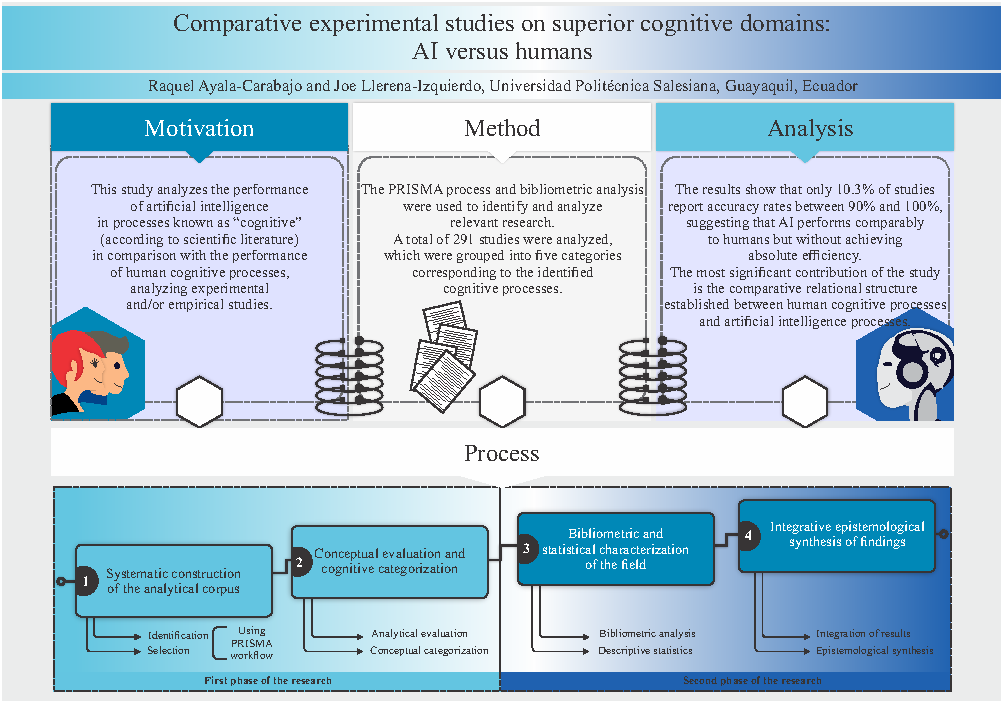
\includegraphics[width=1.0\textwidth]{images/diagrama_metodologia.pdf}
    \label{fig:metodologia}
\end{figure}

Como indica la figura \ref{fig:metodologia} proyecto se llevará a cabo siguiendo una metodología estructurada que abarca desde la revisión exhaustiva de la literatura hasta la documentación final de los resultados \parencite{Zerega-Prado2022}.

\section{Cronograma de actividades}
{\color{magenta}Detalla las actividades generales que se desarrollarán en un tiempo estimado de 400 horas y en los casos necesarios un 10\% de horas adicionales.}

\noindent Se presenta a continuación las actividades a ser desarrolladas durante el proceso de tituación en duración de los meses establecidos y planificados, ver Tabla \ref{tab:cronograma}.

\begin{table}[H]
\centering
\caption{Cronograma de actividades del programa de titulación}
\label{tab:cronograma}
\begin{tabular}{|>{\centering\arraybackslash}p{10cm} | >{\centering\arraybackslash}p{4cm} |}
\hline
\cellcolor{blue!15}\textbf{Actividad} & \cellcolor{blue!15}\textbf{Fecha} \\
\hline
Aprobación del tema por el Consejo de Posgrados & 21/03/2025 \\
\hline
Hito 1 (25\%): Estado del arte & 31/03/2025 \\
\hline
Hito 2 (50\%): Diseño & 14/04/2025 \\
\hline
Hito 3 (75\%): Prueba de concepto & 05/05/2025 \\
\hline
Hito 4 (100\%): Documento final & 26/05/2025 \\
\hline
\end{tabular}
\end{table}

\noindent Además se presenta el plan de actividades determinados por fases del proyecto. Dichas actividades contemplan una fecha inicial y una fecha final, además del nombre de la actividad y quién realiza la actividad mediante el recurso humano, ver Fig. \ref{fig:cronograma1}.

\begin{figure}[H] 
    \centering
    \caption{Actividades dentro del proyecto de titulación, recuerde que es mejor usar una tabla}
    % He quitado width para que scale tome el mando total del tamaño
    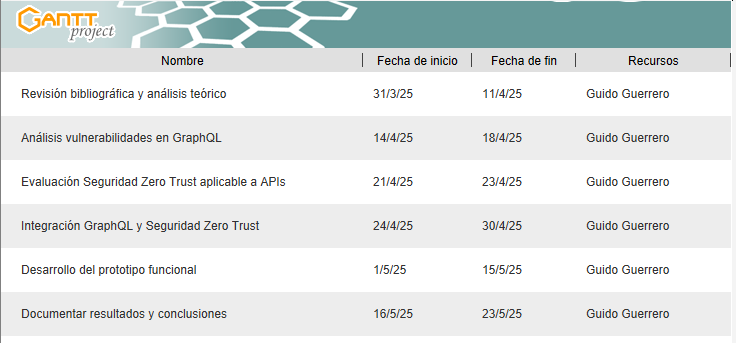
\includegraphics[scale=0.82, trim={0.3cm 0cm 1cm 1.3cm}, clip]{images/Cronograma_Proyecto_MSOFT.png}
    \label{fig:cronograma1}
\end{figure}

\noindent Además se presenta el cronograma con asignaciones de actividades del proyecto realizadas de manera secuencial, cumpliendo con las fechas establecidas y recursos programados con un software como Project (ver Fig. \ref{fig:cronograma}).

\begin{figure}[H] % Entorno para figuras flotantes
    \centering
    \caption{Cronograma Proyecto de Titulación}
    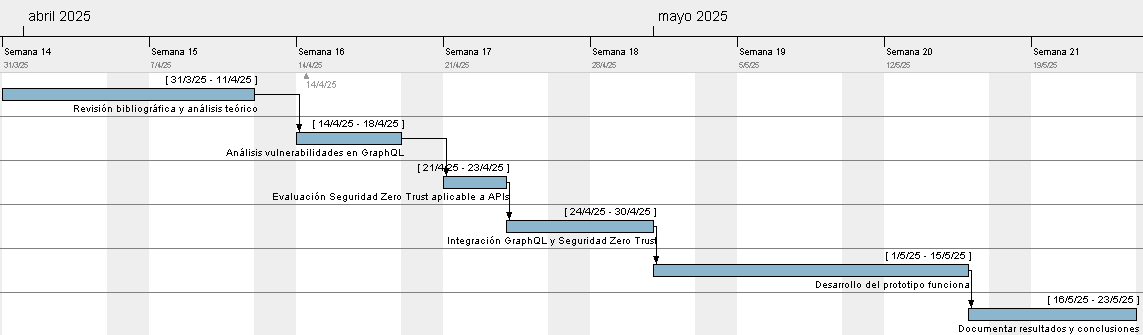
\includegraphics[width=1.\textwidth]{images/Cronograma_Proyecto_MSOFT_Tiempos.png}
    \label{fig:cronograma}
\end{figure}

El cumplimiento de cada fase, propuestas en la figura \ref{fig:cronograma1}, desde la revisión bibliográfica hasta la documentación, permitirá una construcción sólida y coherente del trabajo, asegurando la calidad y pertinencia de los resultados \parencite{sumba2021reflections}. La atención a los plazos, indicados en la figura \ref{fig:cronograma}, por su parte, facilitará una gestión eficiente del tiempo y los recursos, maximizando las posibilidades de éxito en la culminación del proyecto.
Adicionalmente, el cronograma se ajusta al cronograma de Hitos propuesto por la Universidad, esto con el fin de cumplir los plazos establecidos.

\section{Proyectos de investigación vinculados}
{\color{magenta}En caso de existir uno o más proyectos de investigación al que se vincule el trabajo a desarrollar, en esta sección se deberá indicar los datos generales de dichos proyectos, (título y nombre del director del proyecto).}

La presenta propuesta forma parte del proyecto de investigación aprobado denominado: ``Percepciones y dilemas éticos de estudiantes de Ingeniería frente al uso de IA generativa en el aprendizaje'' a cargo del investigador Joe Llerena Izquierdo, coordinador del grupo de investigación GIEACI. La resolución de Consejo de Investigación de Sede es 060-004-2025-06-27. Esta información se expresa para conocimiento de los autores y comprendan que existe un centro de costos para el proyecto y sus productos generados. Adicionalmente se ha firmado la carta de adhesión y entregada al director del proyecto. La línea de investigación a la que perteneces es ``Integración de Tecnologías Emergentes en la Educación en Ingeniería''.

\section{Presupuesto del Proyecto de Titulación}
{\color{magenta}Este apartado incluirá los recursos e información financiera para el Trabajo de Titulación. Si el trabajo pertenece a un grupo de investigación, el grupo asume los gastos de publicación, si se requiere.}

El porcentaje para imprevistos es una estimación y puede ajustarse según se considere necesario. Estos valores son los recomendables por la unidad de titulación y acordados por el grupo de investigación (quién asume los costos si se publica o divulga el artículo) para la debida finalización de la propuesta (ver Tabla \ref{tab:presupuesto}).

\begin{table}[H]
\centering
\caption{Presupuesto Proyecto de Titulación}
\label{tab:presupuesto}
\begin{tabular}{|>{\raggedright\arraybackslash}p{6cm} | >{\raggedright\arraybackslash}p{5cm} | >{\raggedleft\arraybackslash}p{3cm} |}
\hline
\cellcolor{blue!15}\textbf{Concepto} & \cellcolor{blue!15}\textbf{Descripción} & \cellcolor{blue!15}\textbf{Costo (USD)} \\
\hline
Transporte & 6 meses  & 200 \\
\hline
Costos imprevistos & 10\% del costo de desarrollo & 40 \\
\hline
Costo de Internet & 1 mes de servicio a \$30/mes & 30 \\
\hline
Impresión de documentación & Solicitado por la carrera & 160 \\
\hline
\textbf{Total} & & \textbf{430} \\
\hline
\end{tabular}
\end{table}

El presupuesto del proyecto en la Tabla \ref{tab:presupuesto}, estimado en USD 430.00, se compone principalmente de transporte (200 USD), que cubren el tiempo dedicado a la implementación y pruebas del prototipo. Se ha reservado un 10\% (40 USD) para imprevistos, permitiendo cubrir gastos inesperados. Adicionalmente, se incluye un costo mensual de 30 USD por el servicio de internet, importante para la investigación y ejecución del proyecto y un valor de 160 USD para impresiones si son requeridas.

\begin{singlespace} % APA pide las referencias más compactas
%\raggedright % Evita espacios raros entre palabras en la bibliografía

\printbibliography[title={Referencias Bibliográficas}]

{\color{magenta}Este apartado contiene el listado de referencias empleadas para la elaboración del documento, el formato empleados guardará las convenciones de cada área del conocimiento según la carrera.}
\end{singlespace}

\begin{landscape}

\section{Anexos}
\noindent A continuación se muestra una imagen en formato horizontal dentro de landscape, ver Fig. \ref{fig:metodologia2}.

    \begin{figure}[H] % Entorno para figuras flotantes
    \centering
    \caption{Diagrama de flujo de la metodología de investigación para publicación en una revista de alto impacto}
    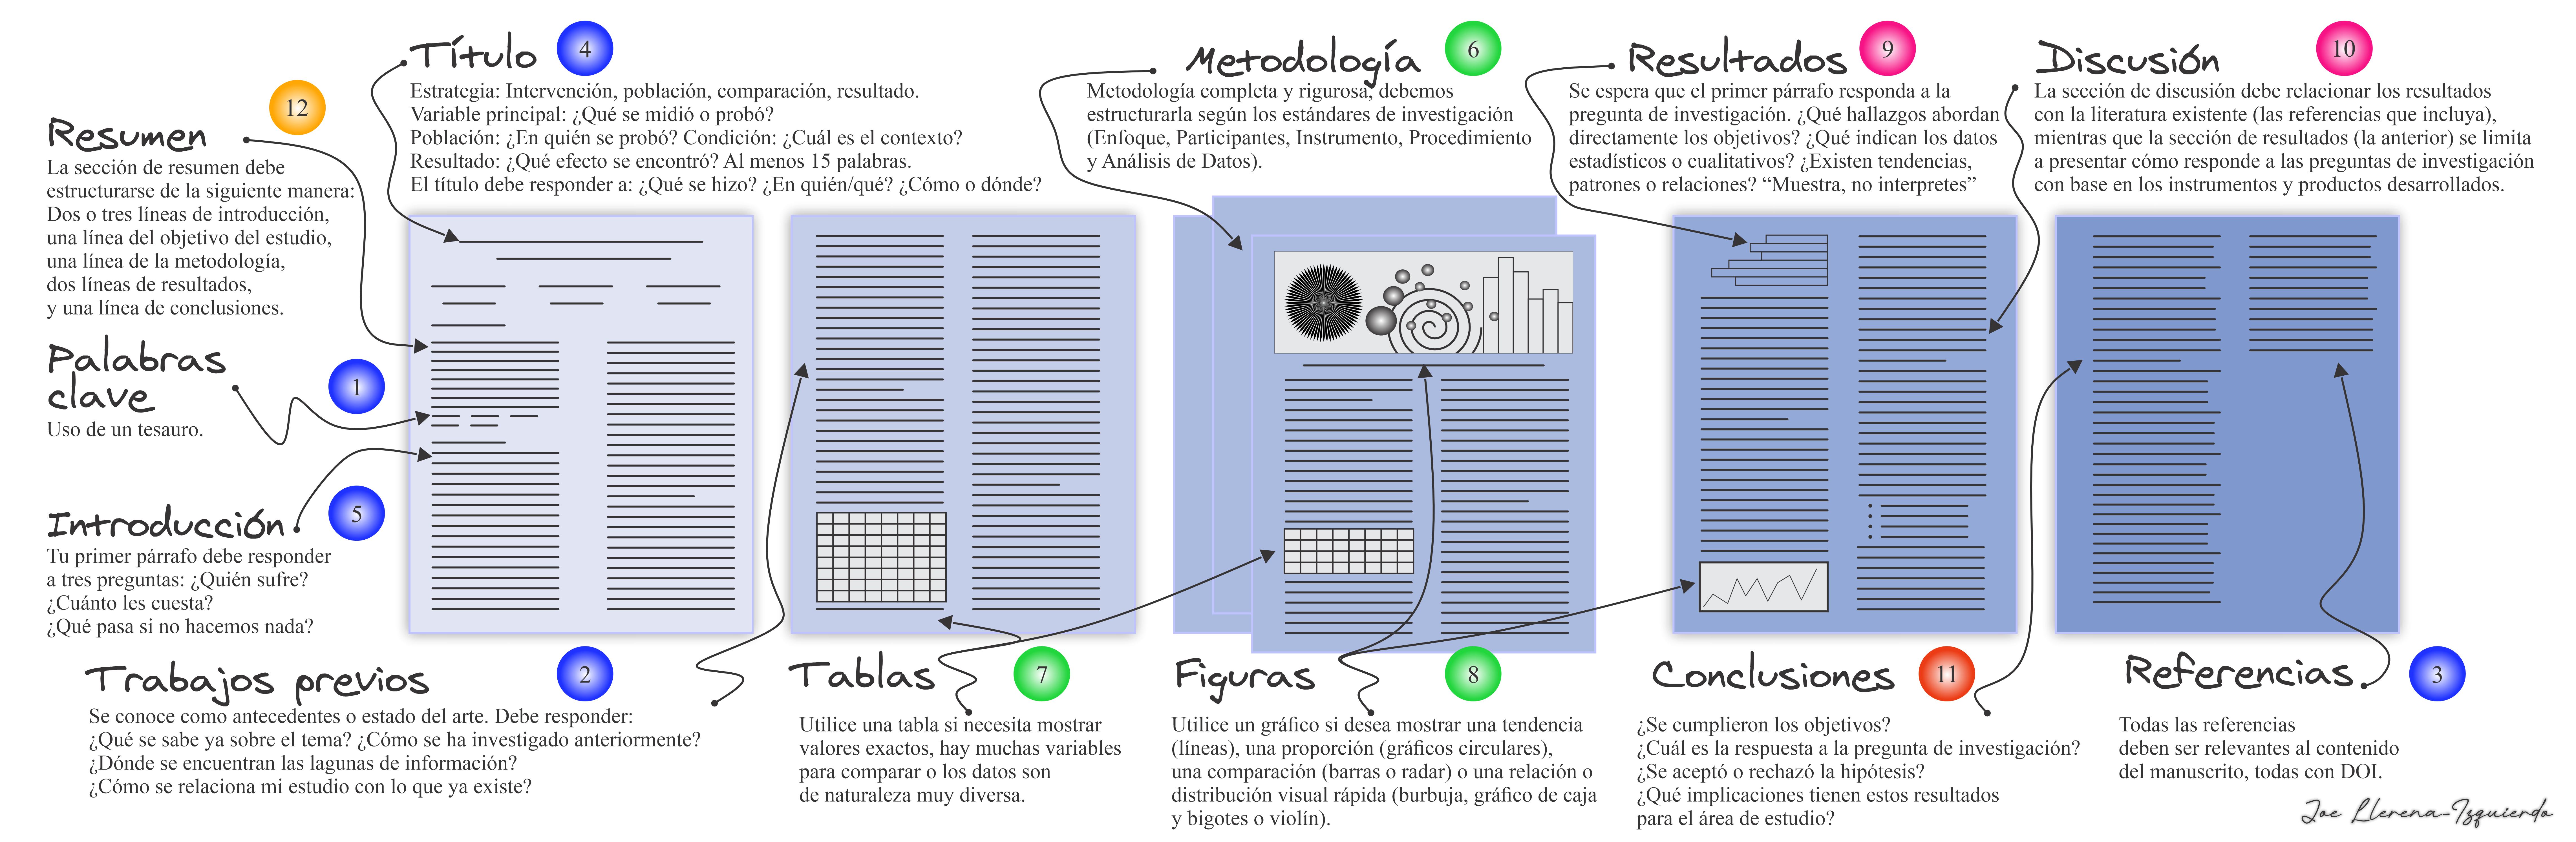
\includegraphics[scale=0.95]{images/diagrama_metodologia.png}
    \label{fig:metodologia2}
\end{figure}
\end{landscape}

\end{document}